\documentclass[12px]{article}

\title{Lezione 27 Geometria I}
\date{2024-05-13}
\author{Federico De Sisti}

\usepackage{amsmath}
\usepackage{amsthm}
\usepackage{mdframed}
\usepackage{amssymb}
\usepackage{nicematrix}
\usepackage{amsfonts}
\usepackage{tcolorbox}
\tcbuselibrary{theorems}
\usepackage{xcolor}
\usepackage{cancel}

\newtheoremstyle{break}
  {1px}{1px}%
  {\itshape}{}%
  {\bfseries}{}%
  {\newline}{}%
\theoremstyle{break}
\newtheorem{theo}{Teorema}
\theoremstyle{break}
\newtheorem{lemma}{Lemma}
\theoremstyle{break}
\newtheorem{defin}{Definizione}
\theoremstyle{break}
\newtheorem{propo}{Proposizione}
\theoremstyle{break}
\newtheorem*{dimo}{Dimostrazione}
\theoremstyle{break}
\newtheorem*{es}{Esempio}

\newenvironment{dimo}
  {\begin{dimostrazione}}
  {\hfill\square\end{dimostrazione}}

\newenvironment{teo}
{\begin{mdframed}[linecolor=red, backgroundcolor=red!10]\begin{theo}}
  {\end{theo}\end{mdframed}}

\newenvironment{nome}
{\begin{mdframed}[linecolor=green, backgroundcolor=green!10]\begin{nomen}}
  {\end{nomen}\end{mdframed}}

\newenvironment{prop}
{\begin{mdframed}[linecolor=red, backgroundcolor=red!10]\begin{propo}}
  {\end{propo}\end{mdframed}}

\newenvironment{defi}
{\begin{mdframed}[linecolor=orange, backgroundcolor=orange!10]\begin{defin}}
  {\end{defin}\end{mdframed}}

\newenvironment{lemm}
{\begin{mdframed}[linecolor=red, backgroundcolor=red!10]\begin{lemma}}
  {\end{lemma}\end{mdframed}}

\newcommand{\icol}[1]{% inline column vector
  \left(\begin{smallmatrix}#1\end{smallmatrix}\right)%
}

\newcommand{\irow}[1]{% inline row vector
  \begin{smallmatrix}(#1)\end{smallmatrix}%
}

\newcommand{\matrice}[1]{% inline column vector
  \begin{pmatrix}#1\end{pmatrix}%
}

\newcommand{\C}{\mathbb{C}}
\newcommand{\K}{\mathbb{K}}
\newcommand{\R}{\mathbb{R}}


\begin{document}
	\maketitle
	\newpage
	\section{Ancora da definire}
	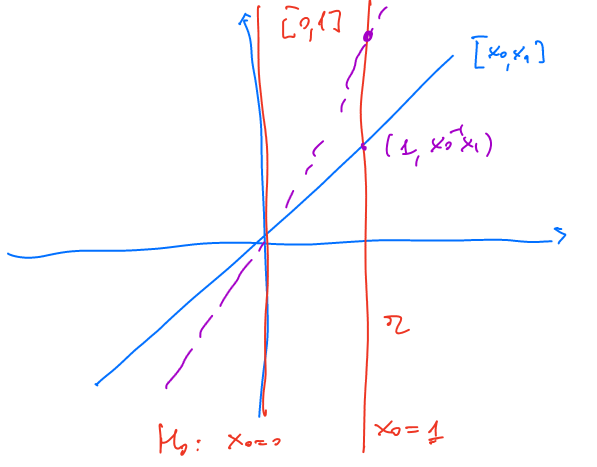
\includegraphics[scale=0.5]{image_1.png}\\
	$\pro^1(\R)=$ rette passanti per $O$  $[x_0,x_1]\in\pro^1(\R)\ \ (\lambda x_0,\lambda x_1)\in\A^2,\ \ \lambda\in\R$\\
	Osserviamo che ogni punto $[x_0,x_1]\in\pro^1\setminus\{H_0\}$ individua una retata parallela ad $r$ (in $\A^2$), che interseca $r$ nell'unico punti $(1,x_0^{-1}x_1)$\\
	(Infatti dobbiamo imporre che $(\lambda x_0,\lambda x_1)$ abbia prima coordinata $1$, cioè $\lambda x_0 = 1$ cioè $\lambda = x_0^{-1}$\\
	Viceversa ogni punto $(1.x)\in r$ appartiene ad un'unica retta per l'origine, quella che corrisponde al punti $[1,x]\in\pro^1\setminus H_0$\\
	In definitiva, abbiamo una corrispondenza biunivoca\\
	\begin{aligned}
		&\pro^1\setminus H_0 \leftrightarrow r\\
		&\pro^1 \leftrightarrow r\cup \{\infty\}\\
		& H_0 \leftarrow \infty \text{ punto all'infinito di } r
	\end{aligned}\\
	La costruzione si generalizza a $\pro^n \leftrightarrow$ rette per l'origine di $\A^{n+1}$\\
	$[x_0,\ldots,x_n]\in\pro^n \leftrightarrow $ rette $\{\lambdax_0,\ldots,\lambda x_{n+1} | \lambda\in \R\}\subseteq \A^{n+1}\ \ \ H_0=\{x_0=0\}$\\
	Consideriamo l'iperpiano affine $A:\{x_0=1\} = \{(1,y_1,\ldots,y_n)\in \A^{n+1}\}$\\
	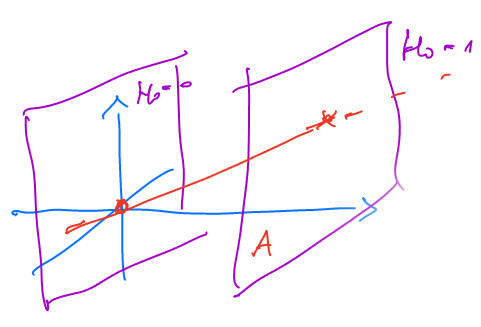
\includegraphics[scale=.5]{Iperpiano_affine_A.jpg}
	\begin{aligned}
		&j: A \rightarrow \pro^n\setminus \{H_0\}\\
		&(1,y_1,\ldots,y_n) \rightarrow [1,y_1,\ldots,y_n]\\
		&y^-1([x_0,\ldots,x_n] = \left[1,\frac {x_1 }{x_0},\ldots, \frac {x_n }{x_0}\right]
	\end{aligned}
	Quindi come sopra, ho una corrispondenza biunivoca
	\[
		A\cup \{H_0\} \rightarrow \pro^n
	.\] 
	Se nella costruzione precedente identificavamo $A$ con $\A^n$ tramite  $(1,y_1,\ldots,y_n) \rightarrow (y_1,\ldots,y_n)$ otteniamo\\
	\begin{aligned}
		&j_0:\A^n \rightarrow\pro^n\seminus\{H_0\}\\
		&j_0(y_1,\ldots,y_n) = [1,y_1,\ldots,y_n] \text{ passaggio a coordinate omogenee rispetto a } x_0\\
		&j_0^{-1}([x_0,\ldots,x_n]) = \left(\frac {x_1}{x_0},\ldots,\frac{x_n}{x_0}\right) \text{ passaggio a coordinate non omogenee rispetto ad } x_0
	\end{aligned}|\\
	ci sono analoghe mappe per ogni $i \ \ 0\leq i \leq n$\\
	\ \\ \hline \ \\
	Modello di  $\pro^1 (\C)$ \\
	$E^3$ spazio euclideo con coordinate $x,y,z$ \\
	\begin{aligned}
		&\pi=\{z=0\} \ \ S^2 = \{(x,y,z)\in E^3|d (\icol{x\\y\\0},\icol{0\\0\\0})=1\}\\
		& N = \icol{0\\0\\1}
	\end{aligned}
	\section{Proiezione stereografica}
	\includegraphics[scale=.3]{Proiezione_stereografica.jpg}\\
	Se $P = \matrice{x'\\y'\\z'}$\\
	 $\overrightarrow{NP}\ \ \begin{cases}
	 	x = x't\\
		t = y't\\
		z = (z-1)t + 1
	 \end{cases}$\\
	 \sigma \matrice{x'\\y'\\z'} = \matrice{\frac{x'}{1-z'}\\\frac{y'}{1-z'}\\0}
	 \textbf{Esercizio}\\
	 $\sigma$ è invertibile con inversa\\
	 \sigma^-1\icol{u\\v\\0}=\matrice{\frac{2u}{u^2+v^2+1}\\\frac{2v}{u^2+v^2+1}\\\frac{u^2+v^2-1}{u^2+v^2+1}}
	 $S^2 \leftrightarrow \pi\cup \{\infty\}$\\
	 identifichiamo  $\pi$ con $\C$ tramite\\
	 \begin{aligend}
		&\pi \ \ \ \ \rightarrow\ \ \ \ \ \C\\
		&\matrice{u&v&0} \rightarrow u + iv
	 \end{aligend}\\
	 Allora abbiamo ottenuto una corrispondenza biunivoca 
	 \[
		 \sigma : S^2 \rightarrow \pro^1{\C} = \C\cup\{\infty\}
	 .\] 
	 \[
	 \sigma(N) =\infty
	 .\] 
	 \[
	 \sigma\matrice{x'\\y'\\z'} = \frac{x'+iy' }{1-z'} \ \ (z\neq 1)
	 .\] 
	 \newpage
	\section{Alcuni degli esercizi svolti a lezione}
	 \textbf{Esercizio}\\
	 Determinare un'equazione cartesiana del piano da $\pro^3(\R)$ passante per  $[1,1,0,1]$ we per i punti impropri delle rette
	 \[
	 r = \begin{cases}
	 	x + y + z-1=0\\
		2x-y-z=0
	 \end{cases}
	 .\] 
	 \[
	 s = \begin{cases}
	 	2x-y-2x+1=0\\
		y+z-1=0
	 \end{cases}
	 .\] 
	 Il punto improprio di $r$ è \begin{cases}
	 	x_1+x_2+x_3-x_0=0\\
		2x_1-x_2-x_3=0\\
		x_0=0
	 \end{cases}\\
	 \begin{aligend}
		& \begin{cases}
			x_1+x_2+x_3=1\\
			3x_1-x_2_x_3=0\\
			x_0=0
		\end{cases}
		\Rightarrow \begin{cases}
			x_1+x_2+x_3=0\\
			3x_1=0\\
			x_0=0\\
		\end{cases}
		\Rightarrow \begin{cases}
			x_0=0\\
			x_1=0\\
			x_2+x_3=0
		\end{cases}
		\Rightarrow  [0,0,-1,-1]\\
		&\text{Per quanto  riguarda s}\\
		& \begin{cases}
			2x_1-x_2-2x_3+x_0=0\\
			x_2+x_3-x_0=0\\
			x_0=0
		\end{cases} \Rightarrow  \begin{cases}
			2x_1-x_2-2x_3=0\\x_2+x_3=0\\
			x_0=0
		\end{cases} \Rightarrow \begin{cases}
			2x_1-x_3=0\\
			x_2+x_3=0\\
			x_0=0
		\end{cases} \\&\Rightarrow  [0,1,-2,2]\\
		&\det\matrice{x_0&x_1&x_2&x_3\\1&1&0&1\\0&0&1&-1\\0&1&-2&2}\\
	&\det\matrice{x_0&x_1&x_2&x_3\\1&1&0&1\\0&0&1&-1\\0&1&0&0}\\
	&\det\matrice{x_0&x_2&x_3\\1&0&1\\0&1&-1}=0
	 \end{aligend}
	 \newpage
	 \section{Dualità}
	 $\pro^V=\pro(V^\star)\ \ \dim\pro=\dim\pro^V$ poichè  $\dim V=\dim V^\star$\\
	 Osserviamo che  $F,F'\in V^\star$ definiscono lo stesso punto in  $\pro^V$ se e solo se  \\$F'= \lambda F\ \ \ \ \lambda\in\K\setminus\{0\}$\\
	 Ma in questo caso $\ker F = \ker F'$\\
	 Ne segue che l'iperpiano  $\ker F$ dipende solo da  $[F]$ Quindi si ha un'applicazione di dualità 
	  \[
		  \delta :\pro^V \rightarrow \{\text{iperpiani di }\pro\}
	 .\] 
	 \[
		 \delta([F]) = \pro(\ker F)
	 .\] 
	 \textbf{$\delta$ è biunivoca}\\
	 è iniettiva perché due funzionali non nulli che hanno lo stesso nucleo sono proporzionali.\\
	 Inoltre l'iperpiano di $V$ è il nucleo di un funzionale, quindi  $\delta$ è suriettiva\\
	 \ \hline \ \\
	 Diciamo che gli iperpiani $H_1,\ldots,H_s$ in $\pro$ sono linearmenete indipendenti se lo sono $\delta^{-1}(H_1),\ldots,\delta^{-1}(H_s)$ \ \\ \hline \ \\
	 Sia $\{e_0,\ldots,e_n\}$ una base di $V$ e sia $\{\eta_0,\ldots,\eta_n\}$ la corrispondente base duale di $V^\star:\eta_i(e_i)=\delta_{e_i}$ 
	 \[
	 H\subseteq \pro^n \ \ a_0x_0+\ldots+a_nx_n=0
	 .\] 
\[
	H = \pro(\ker F) \ \ F\in V^\star \text{ definita :}
\] 
\[
F(\sum^n_{i=1}x_ie_i)=\sum^n_{i=1}a_ix_i
.\] 
Dove le $a_i$ sono le coordinate omogenee di  $[F] $ rispetto al riferimento proiettivo  $\{\eta_0,\ldots,\eta_n\}$\\
In particolare $H=\delta([F]) \ \ \ H=H[a_0,\ldots,a_n]$ \\
\begin{aligend}
	&H_0=H_0[1,\underline{0},\ldots,\underline{0}]=\delta([\eta_0]\\
	&\vdots\\
	&H_n=H_n[0,\ldots,0,1]=\delta([\eta_n])
\end{aligend}
\begin{defi}
	$S\subset \pro$ sottospazio,  $\dim S = k \leq n-1$
	\[
		\bigwedge_1(S) = \{\text{ iperpiani di }\pro \text{ che contengono } S\}
	.\] 
	dove $\bigwedge_1(S)$ è il sistema lineare di iperpiain di centro $S$
\end{defi}
\textbf{Esempi}\\
$\pro=\pro^2 \ \ S = \{Q\}\ \ \\
\bigwedge_1(Q) = \{$ iperpiani di $\pro^2$  che contengono $Q$ = fascio di rette di centro $Q$\\
$\pro=\pro^3 \ \ S = \{r\}\ \ \\ \bigwedge_1(r) = \{$ iperpiani di $\pro^3$ che contengono $r$ = fascio di rette di centro $r$\\
$\pro=\pro^3 \ \ S = \{Q\}\ \ \\ \bigwedge_1(Q) = \{$ iperpiani di $\pro^3$ che contengono $Q$ = stella di rette di centro $Q$\\
\end{document}
